\documentclass[10pt,twocolumn]{paper}
\usepackage{lmodern}
\usepackage{amssymb,amsmath}
\usepackage{ifxetex,ifluatex}
\usepackage{fixltx2e} % provides \textsubscript
\ifnum 0\ifxetex 1\fi\ifluatex 1\fi=0 % if pdftex
  \usepackage[T1]{fontenc}
  \usepackage[utf8]{inputenc}
\else % if luatex or xelatex
  \ifxetex
    \usepackage{mathspec}
  \else
    \usepackage{fontspec}
  \fi
  \defaultfontfeatures{Ligatures=TeX,Scale=MatchLowercase}
\fi
% use upquote if available, for straight quotes in verbatim environments
\IfFileExists{upquote.sty}{\usepackage{upquote}}{}
% use microtype if available
\IfFileExists{microtype.sty}{%
\usepackage{microtype}
\UseMicrotypeSet[protrusion]{basicmath} % disable protrusion for tt fonts
}{}
\usepackage[margin=2cm]{geometry}
\usepackage[unicode=true]{hyperref}
\hypersetup{
            pdftitle={Spatial ecology and movements of wintering White-fronted geese (Anser albifrons)},
            pdfauthor={Pratik R. Gupte},
            pdfborder={0 0 0},
            breaklinks=true}
\urlstyle{same}  % don't use monospace font for urls
\setlength{\emergencystretch}{3em}  % prevent overfull lines
\providecommand{\tightlist}{%
  \setlength{\itemsep}{0pt}\setlength{\parskip}{0pt}}
\setcounter{secnumdepth}{0}
% Redefines (sub)paragraphs to behave more like sections
\ifx\paragraph\undefined\else
\let\oldparagraph\paragraph
\renewcommand{\paragraph}[1]{\oldparagraph{#1}\mbox{}}
\fi
\ifx\subparagraph\undefined\else
\let\oldsubparagraph\subparagraph
\renewcommand{\subparagraph}[1]{\oldsubparagraph{#1}\mbox{}}
\fi
\usepackage{libertine}
\usepackage{textcomp}
\providecommand{\tabularnewline}{\\}
\usepackage{supertabular}
\usepackage{caption}
\usepackage{booktabs}
\usepackage{graphicx}
\usepackage{float}
\usepackage{wrapfig}

\makeatletter
\let\@fnsymbol\@arabic
\makeatother


\title{Spatial ecology and movements of wintering White-fronted geese
(\emph{Anser albifrons})}
\providecommand{\subtitle}[1]{}
\subtitle{Family size dynamics in wintering geese}
\author{Pratik R. Gupte \thanks{International Master in Applied Ecology: Christian-Albrechts-Universit\"{a}t zu Kiel, Universidade de Coimbra, Universit\'{e} de Poitiers}}
\date{}

\begin{document}
\maketitle
\begin{abstract}
The ecology of migratory Arctic-breeding birds on their wintering
grounds is affected by many factors. Hypotheses of interactions between
family size, flock size, foraging site, and age-ratio of wintering geese
have emerged from field observations in western Europe, but are not well
tested. We gathered long-term observation data on flocks of wintering
greater white-fronted geese \emph{Anser albifrons albifrons} from the
Netherlands and northern Germany, and tracked a total of 13 whole
families of the species over three winters (2013, 2014, 2016) with GPS
transmitters. Taking into account effects carried over from the summer,
we explored how the distance of the wintering site from breeding grounds
on Kolguyev Island (69°N, 49°E), number of juveniles in a family, number
of individuals in a flock, and the age-ratio of flocks develop over
time. We related the probability of a family splitting to the number of
times, and the distance that it flew. Families with more juveniles
winter farther west after the first 60 days following autumn arrival,
where flocks are smaller. The number of juveniles in a family, flock
size, age-ratio and the number of families in flocks were well
correlated with the number of days since arrival. Families that
undertook more flights in winter were more likely to split. Our data
suggest that juvenile white-fronted geese separate from their parents
during the winter, and that this species is differentially migratory by
age and social class in both autumn and spring.
\end{abstract}

\renewcommand\dblfloatpagefraction{.95} % for two column documents
\renewcommand\dbltopfraction{.95} % for two column documents
\renewcommand\bottomfraction{.9}
\renewcommand\textfraction{.1}

\setcounter{totalnumber}{50} \setcounter{topnumber}{50}
\setcounter{bottomnumber}{10} \setlength{\textfloatsep}{5pt}
\setlength{\floatsep}{5pt}

\section{Introduction}\label{introduction}

Living in groups entails both costs and benefits for animals. Group
members benefit from more social interactions, and from the increased
sensory and physical capabilities of the group (Krause and Ruxton 2002).
For instance, geese in larger flocks spend less time on the lookout for
predators and have more time to feed (Roberts 1996). Among the costs of
group living is the increased competition for limited resources in
larger groups (Krause and Ruxton 2002). Living in families offers all
the benefits of groups, while costs are shared with relatives.
Individuals may lose some direct fitness in family groups, but this is
offset by the inclusive fitness gained from related group members
(Hamilton 1964, Rodman 1981). Thus animal societies composed of one or
more families are common across taxa, from eusocial insects (Crozier and
Pamilo 1996) to large herbivores (Archie et al. 2006), and cooperative
carnivores (Van Horn et al. 2004).

Many waterbirds, such as geese \emph{Anserini}, live in groups composed
of families. This is most apparent in winter, when families gather to
form foraging and migratory flocks (Elder and Elder 1949). Maintaining
family bonds within flocks confers benefits since families are dominant
over pairs and individuals. Family dominance rank increases with the
number of members, for example in Canada geese \emph{Branta canadensis}
(Hanson 1953), snow geese \emph{Anser caerulscens} (Gregoire and Ankney
1990), and barnacle geese \emph{B. leucopsis} (Loonen et al. 1999). This
allows larger families to occupy optimal foraging positions in flocks at
lesser cost, and win access to better resources (Black et al. 1992).
Both parents and offspring benefit from family bonds maintained across
seasons, as juveniles gain access to more uninterrupted feeding in
winter, and parents gain dominance rank (Black and Owen 1989). Parents
of some species benefit in summer from the presence of nest-attending
sub-adults (Fox and Stroud 1988); barnacle geese that are associated
with their young through a winter, for example, are more likely to
return with a brood the next year (Black and Owen 1989).

From the summer breeding season, through autumn migration, on the
wintering grounds, and often up to and beyond the return spring
migration, goose family bonds are affected by a number of factors. A
combination of weather conditions and levels of summer predation on the
breeding grounds plays an important role in the success of a pair
hatching and fledging young (Summers 1986, Dhondt 1987, Summers and
Underhill 1987, Bêty et al. 2004). The effect of summer predation linked
to the abundance, or lack thereof, of lemmings and voles
\emph{Arvicolinae} has historically been significant enough in some
species to be detectable at the population level in winter (Summers and
Underhill 1987, Jongejans et al. 2015). Autumn migration takes a further
toll in long-distance migrants, especially on yearling birds (Owen and
Black 1989, Francis et al. 1992). In spring, juvenile geese become
independent of parents (Prevett and MacInnes 1980, Johnson and Raveling
1988, Black and Owen 1989), being chased off in some species (Black and
Owen 1989, Poisbleau et al. 2008). However, some juveniles may remain
associated with parents through the spring migration and on the breeding
grounds, where they help fend off predators and competitors (Ely 1979).

The development of family bonds in winter, however, is not fully
understood, and appears to be variable. Small species, such as Ross'
geese \emph{A. rossii}, show weak family bonds in winter, perhaps
because these confer no dominance benefit against much larger snow geese
with which they form mixed flocks (Jónsson and Afton 2008). Similarly,
cackling geese \emph{B. hutchinsii} grazing in large, dense flocks show
weak pair and family associations in winter which strengthen as they
move to areas with fewer geese (Johnson and Raveling 1988). In contrast,
larger taxa such as giant Canada geese \emph{B. canadensis maxima} and
Greenland white-fronted geese \emph{A. albifrons flavirostris} show
strong, extended family bonds (Warren et al. 1993). In general, small,
grazing species tend to dissolve families in winter (Johnson and
Raveling 1988), while large species that need to teach juveniles to
locate and handle high quality foods tend to maintain them longer
(Warren et al. 1993, Kruckenberg 2005).

The question of what space-use and movement decisions families make on
the wintering grounds has also not been well explored, especially in the
context of accompanying juveniles. Some effect is expected, since the
flight of dark-bellied brent geese \emph{Branta b. bernicla} on autumn
migration is affected by the presence of juveniles (Green and Alerstam
2000). Like other birds, geese can be differentially migratory with
different population classes occupying different wintering areas
(Cristol et al. 1999). For example, the white and blue morphs of snow
geese show longitudinal separation during migration (Cooke et al. 1975).
Further, more juveniles of Pacific black brent geese \emph{B. b.
nigricans} winter closer to the breeding grounds (Schamber et al. 2007).
However, how the number of juveniles in a family influences where it
winters is not well understood.

Though the maintenance of family bonds in geese is beneficial,
separation of juveniles from parents is the norm. The mechanistic causes
underlying family separation are not well studied. In wintering snow
geese, family separation is held to be caused by a lack of coordination
between members during chaotic take-offs in large flocks, and is thus
seen as accidental (Prevett and MacInnes 1980). Separated birds attempt
to locate their families, and similar behaviour is observed in Canada
geese (Elder and Elder 1949). Investigating the role of flight events in
family size dynamics requires accurate, fine-scale knowledge of
individual positions, and obtaining such data for whole families of
highly mobile species has historically presented challenges.

Greater white-fronted geese \emph{Anser albifrons albifrons}, hereafter
white-fronted geese, are among the most abundant geese wintering in
continental western Europe (Madsen et al. 1999), and offer an
interesting opportunity to investigate the wintertime dynamics of goose
families. Accounts suggest that in the Baltic-North Sea flyway
population of white-fronted geese (Philippona 1972), larger families
winter farther west than smaller ones. Further, these families are
observed in smaller flocks, but this may be an artefact of smaller
flocks being observed farther west. Family bonds reportedly weaken
within winters, contrary to the trend for families of large taxa to stay
together through the winter, and sometimes beyond (Warren et al. 1993,
Kruckenberg 2005). We draw on long-term field observations and high
frequency GPS tracks of whole families of white-fronted geese from their
wintering grounds in the Netherlands and northern Germany (Mooij 1991,
Madsen et al. 1999, Fox et al. 2010) to test the hypotheses that:
\emph{1.} Larger families winter to the west, farther from the breeding
grounds \emph{2.} Larger families winter in smaller flocks, \emph{3.}
Families decrease in size over the winter, \emph{4.} Family size in
winter shows effects carried over from summer predation and autumn
migration, and \emph{5.} Family separation is predicted by the number
and frequency of flights, and the time since take-off.

\section{Methods}\label{methods}

\subsubsection{Observation data}\label{observation-data}

We censused flocks of wintering white-fronted geese on their wintering
grounds in western Europe by direct counts using field scopes. Observers
counted the total number of birds (flock size), and identified first
winter juveniles (juveniles) among them from plumage characteristics
(dataset \emph{A}). Families were identified by characteristic
behaviours, and were defined as pairs with at least one associated
juvenile (successful families). The number of juveniles associated with
a pair, and the number of families of each size were recorded in a
subset of censused flocks (dataset \emph{B}). Censuses occurred at both
fixed points and \emph{ad hoc} sites. Observers further reported
sightings of individual geese marked with numbered plastic neckbands,
including their position and social class, online (\emph{geese.org},
dataset \emph{C}). These data included records of single geese and pairs
without accompanying juveniles (unsuccessful families). To estimate the
effect of migration mortality, we censused geese on the breeding grounds
on Kolguyev Island (ca. 69°N, 49°E) in August 2016, approximately 1
month prior to the autumn migration, noting the size and social
composition of all groups of geese seen (dataset \emph{D}). Both
successful and unsuccessful families were recorded.

Winter data were filtered to exclude records outside the spatial (2 -
10°E, 50 - 54°N) and temporal (autumn 2000 - spring 2017, breeding years
2000 - 2016) limits of our study. Records of unpaired neckbanded geese
without juveniles were also removed. We obtained 7,149 flock counts from
75 observers at 123 geocoded sites (automated using Kahle and Wickham
2013). Of these, 1,884 flocks counted by 17 observers at 65 sites held
51,037 successful families. A further 10,635 marked geese were observed
at 8,416 sites. Observations of marked geese did not include details on
habitat type, flock size and observer. We obtained 116 records of goose
families from Kolguyev Island.

\subsubsection{Whole family tracking}\label{whole-family-tracking}

We also collected half-hourly positions of a total of 13 goose families
(13 adult pairs, 38 juveniles) fitted with GPS transmitters (2013, n =
3, 2014, n = 4: e-obs GmBH, \& 2016, n = 6: madebytheo) (dataset
\emph{E}). In addition, 2016 transmitters collected short 0.5 Hz bursts
of position data from take-off events. Families fitted with GPS
transmitters were tracked within the study site (2 - 10°E, 50 - 54°N) in
winter (pre-April 01) for 78 days on average (range: 34 - 135). For all
families, we identified the day and position where splits were first
detected as a decrease in the number of birds within a 250m radius of a
designated reference bird (see Fig. 1). Before analysing the daily
probability of splitting, we defined `flights' as displacements of
greater than 1km, and counted their number and daily frequency. For 2016
families, we identified the half-hour when they split, and identified
take-offs as 0.5 Hz records with a ground speed above 2 m/s. We then
calculated the time since the last take-off at each half-hour.

\begin{figure*}
\centering
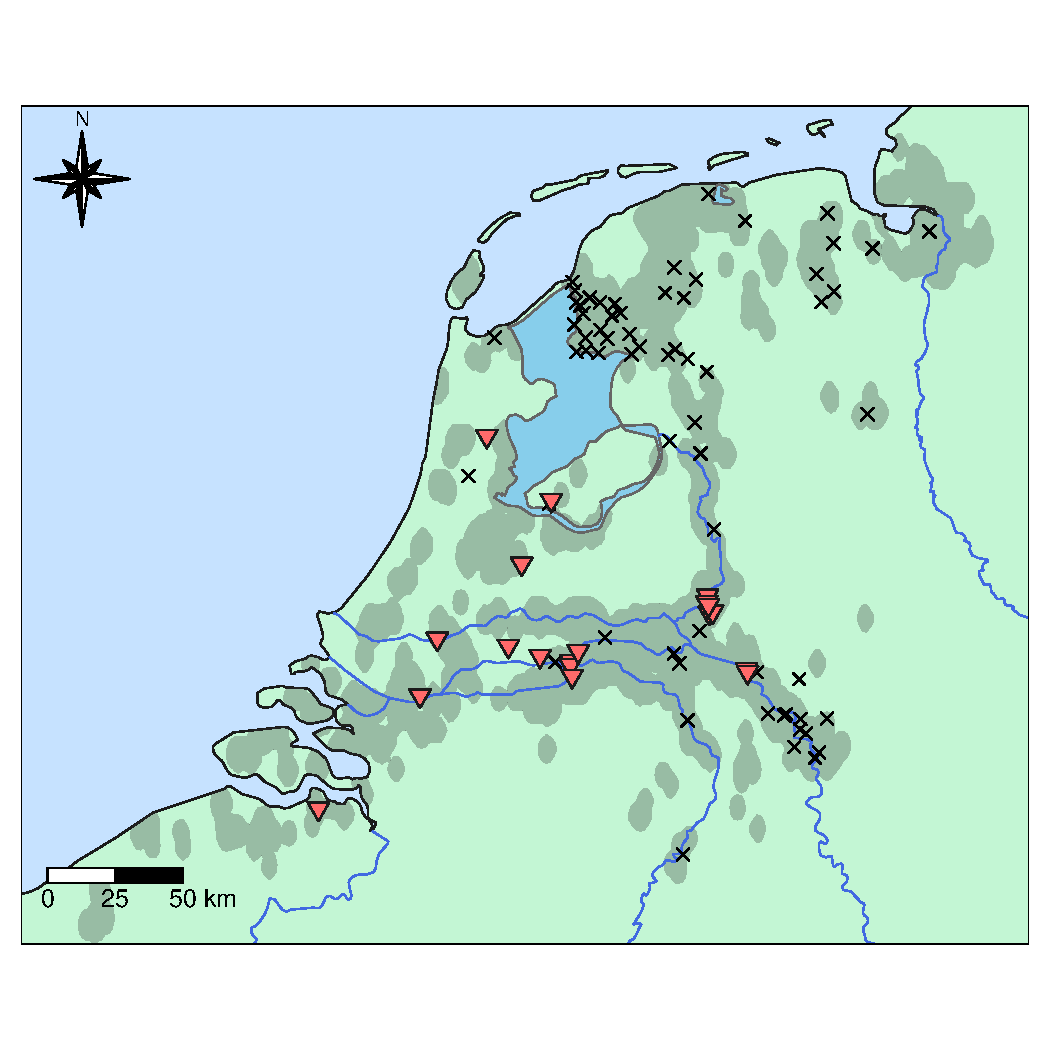
\includegraphics[width = 0.8\linewidth]{datamap.pdf}
\caption{{\small \emph{a.} Wintering grounds of greater white-fronted geese \emph{Anser a. albifrons} in the Netherlands and northern Germany, with 65 sites (dots) where 51,037 successful families in 1,884 flocks were recorded.
21 splits (diamonds) were observed in 13 GPS tracked families. Shaded
area bounds 10,635 observations of marked geese. Observations correspond well with major rivers and waterbodies, marked in blue. Data were collected
from 2000 - 2017. \emph{b.} Breeding grounds in Russia (ellipse) with Kolguyev
Island (dot) and general direction of migration (arrow) to wintering area
(rectangle).}}

\end{figure*}

\begin{table*} \centering
\begin{tabular}{c*5l}
\toprule
Dataset & Type & Records & Sites & Spatial extent (\textdegree ) & Temporal extent (yr)\\
\midrule
A & Flock counts & 7,149 & 123 & 4.0 - 8.8 E, 51.1 - 53.4 N & 2000 - 2017 \\
B & Family counts & 51,037 & 65 & 4.8 - 7.3 E, 51.1 - 53.4 N & 2000 - 2017 \\

C & Marked geese & 10,635 & 8,416 & 2.7 - 9.7 E, 50.9 - 53.9 N & 2000 - 2017 \\
D & Family counts & 116 & 26 & 49 E, 69 N & 2016 \\
E & Family GPS tracks & 13\textsuperscript{a}; 32,630\textsuperscript{b} & 32,630 & 3.9 - 7.9 E, 51.3 - 54.3 N & 2013\textsuperscript{c}, 2014\textsuperscript{d}, 2016\textsuperscript{e} \\\midrule

\multicolumn{6}{l}{\emph{a: Number of families, b: Number of half hourly positions, c: 3 families, d: 4 families, e: 5 families}}\\
\bottomrule
\end{tabular}
\caption{{\small Summary of filtered datasets.}}
\end{table*}

\subsubsection{Supplementary data}\label{supplementary-data}

To relate observation data to migration timing, we collected daily
records (n = 6,266) of flock flight intensity pooled over 84 spring and
180 autumn (overlap = 72) Trektellen sites (Van Turnhout et al. 2009) in
the Netherlands. We excluded flight activity records from sites close to
night roosts, and records which did not match the direction of migration
appropriate to the season. We used these data to find the beginning and
end of each goose winter across the study period. We took the goose
winter to begin with the first mass arrival of geese in autumn, and to
end with the last mass departure in spring.

Following previous studies (Jongejans et al. 2015) we estimated an index
of summer predation for the breeding grounds of this population from
rodent abundance data (\emph{arcticbirds.net}). We calculated a pooled
mean of 0 - 2 (low - high) lemming indices from sites in the region,
taking care to include a value of 0 in each year to reflect absence of a
lemming cycle in the core breeding area on Kolguyev Island. The index
takes into account the cyclical change in lemming abundance, with higher
values when lemming abundance had decreased from the previous year
reflecting the increased predation pressure on Arctic birds from
abundant predators switching to alternative prey (see Dhondt 1987).

\subsubsection{Analyses}\label{analyses}

We first tested whether (\emph{1.}) the number of juveniles, which
determines family size, was correlated with the distance from the
breeding grounds at which families were observed. Here, we used datasets
\emph{B} and \emph{C}. Using dataset \emph{B}, we tested whether
(\emph{2.a.}) the number of juveniles in a family, and (\emph{2.b.}) the
total number of successful families was explained by a combination of
flock size, the number of days since the arrival of geese in autumn, and
the level of summer predation. We also tested whether (\emph{2.c}) the
number of juveniles in families was different 1 month prior, and up to 2
months after autumn migration in 2016 using datasets \emph{B, C} and
\emph{D}. To place these results in context, we searched for (\emph{3.})
an effect on flock size (from dataset \emph{A}) of distance from the
breeding grounds, the number of days since arrival, and summer
predation, and examined whether (\emph{4.}) the proportion of juveniles
in flocks (from dataset \emph{A}) was explained by the flock size,
distance from the breeding grounds, number of days since arrival, and
summer predation (see Tab. A1).

Further, using dataset \emph{E} we examined whether (\emph{5.a.}) the
split probability (no-split or split, binomial distribution) each day
was predicted by the days since arrival, the number of flights that day,
the cumulative number of flights until that day, the distance travelled
that day, the cumulative distance travelled until that day, and the
family size on that day. For the 2016 families we tested (\emph{5.b.})
the half-hourly split probability in relation to the time since the last
take-off and the distance travelled in the previous half hour (see Tab.
A2).

All analyses were performed in the \emph{R} environment (R Core Team
2017) (see Tab. A1). We used a simple Poisson-error generalised linear
model to test \emph{2.c}. We used Poisson \emph{lme4} (Bates et al.
2015) generalised linear mixed models (GLMMs) to test \emph{1, 2.a}, and
\emph{3}, and binomial-error GLMMs for \emph{5.a} and \emph{5.b}. In
\emph{2.b} and \emph{4}, we used \emph{mgcv} (Wood 2013) Poisson
(\emph{2.b}) and binomial (\emph{4}) generalised additive mixed models
(GAMMs) to include smooth functions of the flocksize (in \emph{2.b}) and
the number of days since winter (in \emph{4}) as predictors. We included
some covariates as independent random effects, and effects included in
models were dependent on their availability in the datasets used (see
Tab. A1). We assessed the importance of each predictor using Type II
Wald χ\textsuperscript{2} tests, and effect sizes using Cohen's
\emph{f\textsuperscript{2}} (see Appendix 2).

\section{Results}\label{results}

\subsubsection{Data filtering}\label{data-filtering}

Flock count data from 16 breeding years and subsequent winters yielded a
mean 420 flock counts per year (range: 67 (2001) - 672 (2005)). Except
one record in August 2016, spring (Aprils, n = 24) and early autumn
(Septembers, n = 76) had the fewest records, with most observations from
winter (October - January, 81\%, n = 5,785). Observations declined over
February (11\%) and March (6.8\%). The mean flock size was 712 (range: 2
- 20,000), with a mean proportion of first-winter birds of 0.18 (range:
0 - 0.87). Flocks in which families were counted held on average 540
birds (range: 3 - 11,000), with an average of 27 families (range: 1 -
333) accompanied by a mean of 1.78 juveniles (range: 1 - 10). On
average, marked geese were observed 626 times overall (range: 62 - 1143)
were observed each year, accompanied by 0.59 juveniles (range: 0 - 11)
(see Appendix 1, Figs. A1, A2). Families on Kolguyev Island in 2016 had
a mean of 2.26 juveniles (range: 0 - 6).

Families fitted with GPS transmitters travelled on average 11 km each
day (range: 0 - 306). At the daily scale, families travelled a distance
\textgreater{} 1km a mean of twice per day (range: 0 - 10), and on
average 98 times (range: 63 - 367) over the tracking period. In 2016
families, take-offs occurred on average 5 times (range: 1 - 15) a day,
and 470 times (range: 328 - 659) over the tracking period. 21 family
splits occurred in the 13 families tracked and were not restricted to
juveniles. Flock flight intensity reached the 90th percentile for
autumns between September 26 and October 30, and was at the 90th
percentile for the last time between March 03 and April 01. Representing
the arrival and departure of geese, respectively, this resulted in a
mean goose winter of 165 days. Lemming abundance from the breeding
grounds transformed into a predation index ranged between 1.17 and 1.9,
with very low variance between years (σ\textsuperscript{2} = 0.048).

\subsubsection{Juveniles and wintering site
choice}\label{juveniles-and-wintering-site-choice}

We found no influence of the number of juveniles in a family on how far
from the breeding grounds a family wintered in the first sixty days
after arrival (dataset \emph{B}: successful families in flocks, and
\emph{C}: families of marked geese, model \emph{1}, χ\textsuperscript{2}
B = 1.135, p B = 0.286, χ\textsuperscript{2} C = 2.007, p C = 0.157, see
Fig. 2). Later in the winter, larger families from dataset \emph{B}
(successful families in flocks) wintered farther west
(χ\textsuperscript{2} = 4.194, p = 0.041), while dataset \emph{C}
(families of marked geese) did not reveal any influence of juvenile
number on wintering site (χ\textsuperscript{2} = 0.27, p = 0.6033).

\begin{figure}
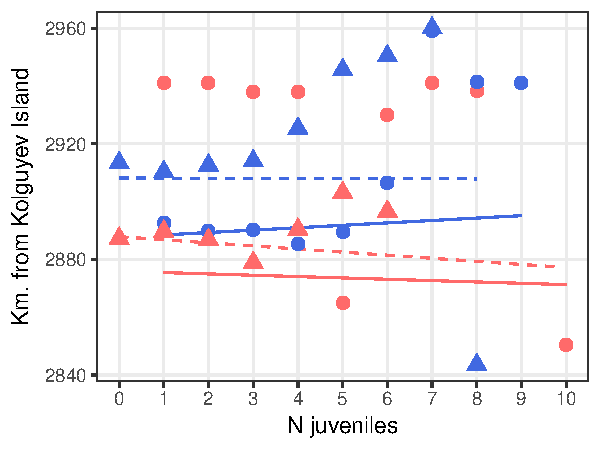
\includegraphics[width = 1\linewidth]{dist_fam.pdf}
\caption{{\small GLMM fits (lines), and mean distance of wintering sites from Kolguyev Island (symbols) per number of juveniles in a family. Data and fit for
records from \textless{} 60 days after arrival are shown in red; data and fit for records \textgreater{} 60 days after arrival are in blue.
Triangles \& dotted lines represent data from marked geese (dataset \emph{C}), circles and solid lines family counts (dataset \emph{B}.}}
\end{figure}

\subsubsection{Family size in winter}\label{family-size-in-winter}

The number of juveniles in a family (dataset \emph{B}: successful
families in flocks, model \emph{2.a}) decreased through the winter
(χ\textsuperscript{2} = 74.166, p \textless{} 0.001, see Fig. 3), but
was insensitive to flock size (χ\textsuperscript{2} = 0.270, p = 0.6033)
and summer predation (χ\textsuperscript{2} = 0.337, p = 0.562, see Fig.
A3). Family sizes of marked geese (dataset \emph{C}: families of marked
geese, model \emph{2.a} adapted) decreased over time
(χ\textsuperscript{2} = 19.936, p = \textless{} 0.001, see Fig. 3), but
showed an increase with the level of summer predation
(χ\textsuperscript{2} = 12.935, p \textless{} 0.001, see Fig. A3). We
tested whether the exclusion of unsuccessful pairs from family counts in
flocks biased the data by similarly excluding such records from
observations of marked geese. We confirmed this bias in sampling method
by failing to find any effect of summer predation after excluding
unsuccessful pairs from data \emph{C} (χ\textsuperscript{2} = 0.1321, p
= 0.716, see Fig. A3). The number of successful families in flocks
increased with flock size (χ\textsuperscript{2} = 7162, p \textless{}
0.001), and the number of days since goose arrival in autumn
(χ\textsuperscript{2} = 171.3, p \textless{} 0.001, see Fig. 4), but was
unaffected by summer predation (χ\textsuperscript{2} = 0, p = 0.98).
Further, there were more successful families in flocks farther from the
breeding grounds (χ\textsuperscript{2} = 12.73, p = 0.0004, see Fig. 5).

\begin{figure}
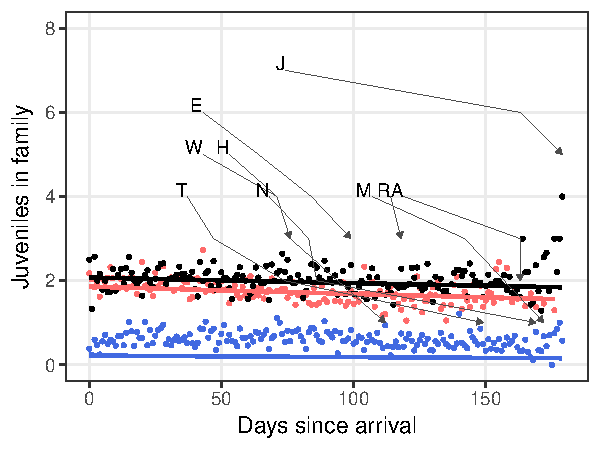
\includegraphics[width = 1\linewidth]{fam_time.pdf}
\caption{{\small GLMM fits (lines) and mean number of juveniles per family on each day since goose autumn arrival pooled across years (dots). Successful families in flocks (dataset \emph{B}) are shown in red, and families of marked geese (dataset \emph{C}) are shown in blue. Arrows show development of size of 9 GPS tracked families that underwent splits.}}
\end{figure}

\begin{figure}
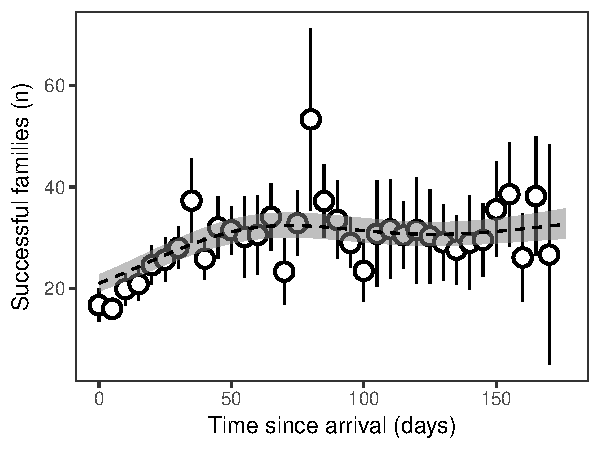
\includegraphics[width = 1\linewidth]{nfams_time.pdf}
\caption{{\small GAMM partial fit (line) and mean number of successful families in
white-fronted goose flocks on each winter day, pooled across all winters
(circles). 95\% confidence interval is shaded grey.}}
\end{figure}

\begin{figure}
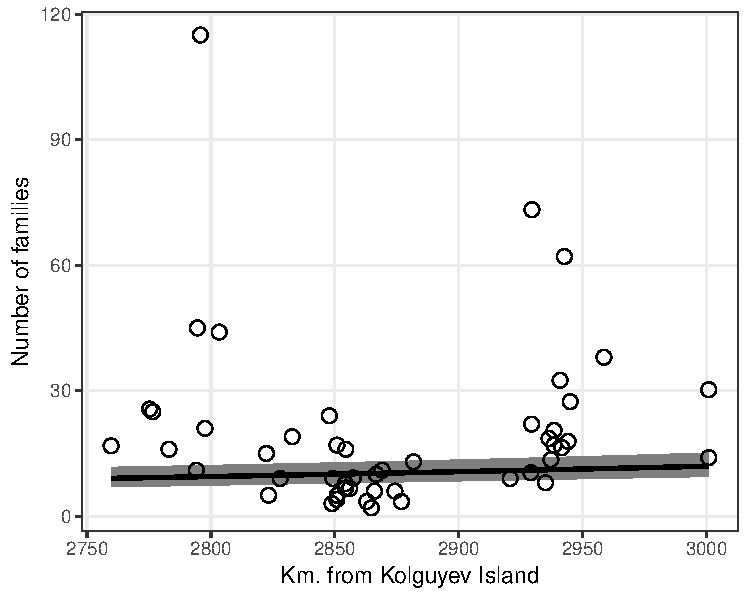
\includegraphics[width = 1\linewidth]{nfams_dist.pdf}
\caption{{\small GAMM fit (line) and mean number of successful families in
white-fronted goose flocks at each site (circles, n = 49) as a function
of its distance from the Kolguyev Island. 95\% confidence interval is
shaded grey.}}
\end{figure}

\subsubsection{Family size and autumn
migration}\label{family-size-and-autumn-migration}

Families of geese observed approximately one month pre-migration on
Kolguyev Island (dataset \emph{D}) had significantly more juveniles than
successful families (dataset \emph{B}) in flocks (GLM, z = -4.285, p
\textless{} 0.001) and families of marked geese (dataset \emph{C}) (GLM,
z = -14.511, p \textless{} 0.001) recorded in the first two months
following the population's arrival on the wintering grounds.

\subsubsection{Flock size in winter}\label{flock-size-in-winter}

Flocks were significantly smaller farther from the breeding grounds
(χ\textsuperscript{2} = 66599, p = \textless{} 0.001, see Fig. A5), and
grew slightly over the winter (χ\textsuperscript{2} = 4975, p
\textless{} 0.001). Within flocks, juvenile proportions increased
through the winter (χ\textsuperscript{2} = 19.43, p = 0.001, see Fig.
A4), and decreased with increasing flock size (χ\textsuperscript{2} =
5.921, p = 0.015, see Fig. A6), but did not show any effect of distance
from the breeding grounds (χ\textsuperscript{2} = 1.015, p = 0.314), or
of summer predation (χ\textsuperscript{2} = 0.021, p = 0.883).

\subsubsection{Probability of family
splits}\label{probability-of-family-splits}

The daily probability of families separating (see Fig. 6) was
significantly lower later in the winter (χ\textsuperscript{2} = 8.314, p
= 0.004), and lower in larger families (χ\textsuperscript{2} = 11.41, p
\textless{} 0.001). There was no effect of the daily number of flights
(χ\textsuperscript{2} = 0.018, p = 0.893), nor the daily distance moved
(χ\textsuperscript{2} = 2.99, p = 0.083). Split probability was higher
in families that made cumulatively more flights over the period leading
up to the split (χ\textsuperscript{2} = 143.23, p \textless{} 0.001),
but decreased in families that moved a shorter cumulative distance over
the days leading up to splits (χ\textsuperscript{2} = 182.63, p
\textless{} 0.001). At the half-hour scale, split probability increased
with time since the previous take-off (χ\textsuperscript{2} = 6.07, p =
0.014), but was not related to the distance travelled in the previous
half hour (χ\textsuperscript{2} = 0.389, p = 0.533).

\begin{figure}
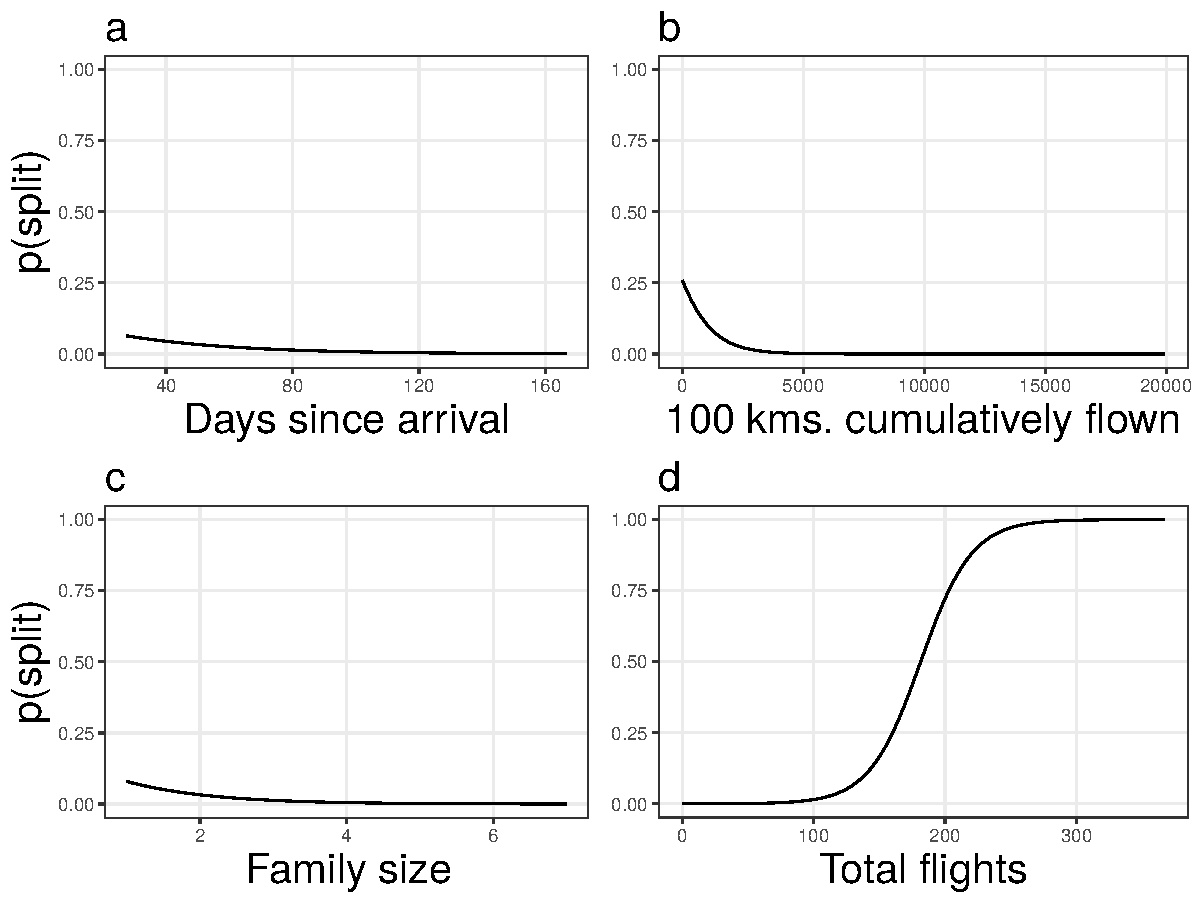
\includegraphics[width = 1\linewidth]{split_dayprob.pdf}
\caption{{\small GAMM partial fits (lines) for (a) days since arrival, (b) cumulative number of flights over winter, (c) number of juveniles, and (d) cumulative number of displacements of more than 1000 km.}}
\end{figure}

\section{Discussion}\label{discussion}

We studied how the size of white-fronted goose families is related to
where, when and with how many flockmates they are seen in the wintering
grounds. We found support for the effect of the size of successful
families on how far they migrate from the breeding grounds, but only
later in winter. Further, the number of successful families in flocks
was higher in the west. We also confirmed that family size decreases
over the winter, but found that it is insensitive to flock size, and
shows mixed responses to summer predation. Families are less likely to
split later in winter, and with increasing family size. We found only
indirect evidence that flights are responsible for family splits in
winter. We showed that flocks are smaller farther from the breeding
grounds, and found that they increase in size over the winter.
Additionally, larger flocks have more successful families. The
proportion of first year birds in flocks is lower in larger flocks, but
increases as winter progresses.

Social class has been found in previous studies to influence geese's
selection of wintering sites, with dominant social units displacing
subordinate ones from optimal wintering locations (Vangilder and Smith
1985, Schamber et al. 2007). Our finding that larger families winter to
the west of the study area is similar to one found by Jongejans et al.
(2015). It fits the idea that dominant social units occupy optimal
wintering sites if the spatial distribution of white-fronted goose
families reflects habitat suitability. Arctic geese can exploit most of
the highly productive landscape in western Europe, and have become
tolerant of human disturbance and previously deterrent structures such
as wind turbines (Madsen and Boertmann 2008, Fox and Madsen 2017). Any
habitat selection is thus likely to be against conditions that impede
foraging, such as snow and ice cover coupled with strong winds
(Philippona 1966). Geese tolerate snow depths of ca. 15cm, conditions in
excess of which are not noted in the Netherlands before midwinter
(Philippona 1966), and have become rare within the study period. Western
areas near the North Sea coast may be expected to benefit from its
moderating effect on temperature, with fewer instances of conditions
that geese would prefer to avoid. This could explain why adults with
juveniles would winter there after midwinter. The movement of geese to
the south later in winter has previously been reported, with peak counts
of white-fronted geese in the Netherlands in November (Hornman et al.
2015), but only in January in Belgium (Devos and Kuijken 2010), lending
support to our finding.

Juvenile independence has been reported across goose taxa (eg. Prevett
and MacInnes 1980, Johnson and Raveling 1988, Black and Owen 1989) as
being concurrent with the arrival of spring. Previous studies have shown
that spring copulation in the breeding pair triggers juvenile departure
(Fischer 1965, Prevett and MacInnes 1980). We find support for the
hypothesis that the number of juveniles with adults decreases through
the winter. The dissociation of juveniles from parents should result in
some pairs losing the single juvenile associated with them, thus
reducing the number of successful families counted in flocks over the
winter. Our finding that the number of families seen in flocks increases
as winter progresses contradicts this expectation. An explanation could
be that social class predicts variation in spring migration timing, with
families leaving later than pairs without juveniles. This is already
known from the autumn migration, with families arriving later than
non-breeding birds (Jongejans et al. 2015). However, previous studies
have not found such an effect in grey geese in spring (Madsen 2001, Bêty
et al. 2004).

Summer predation, in turn driven by the cyclical abundance of Arctic
rodents, is another mechanism by which the populations of
Arctic-breeding birds, including geese, are suggested to be regulated
prior to migration (see Summers 1986, Summers and Underhill 1987,
Blomqvist et al. 2002). Recent studies however indicate that since the
2000s, the breeding success of Baltic-North Sea flyway white-fronted
geese no longer seems to be correlated with summer predation (Jongejans
et al. 2015). This may explain our findings that the number of juveniles
in successful families is not affected by summer predation intensity.
Notably, the Pannonian population of white-fronted geese, which breeds
on the Taimyr Peninsula, continues to show a correlation with predation,
and by extension with rodent abundance. It has been suggested that more
Baltic-North Sea white-fronted geese now breed on Kolguyev Island where
they experience a constant level of predation, since the island lacks
lemmings and associated phenomena (Kruckenberg et al. 2008). A large
Arctic breeding range (45°E - 85°E, ca. 1,800km, Baltic-North Sea
population) likely means that variation in predation pressure is lost
due to year-wise averaging across sites. Future models could correct for
this by accounting for predation at the summering site of each family
observed in winter.

Lemming cycles in northern Russia appear to be faltering and this could
also explain why cyclicity in goose breeding success has been reduced
(Nolet et al. 2013). Angerbjörn et al. (2001) have shown that the
cyclicity of lemming populations in Fennoscandia has been previously
disrupted and re-established in the later-19th and 20th centuries. This
lends support to the idea that northern Russian lemming cycles might be
undergoing similar temporary disruption, following which they could be
restored. The increase in the number of juveniles seen with marked geese
during years of increased predation could suggest that facing high
predation pressure, geese either fledge large families or fail entirely.
This could be the case if geese more effective at repelling predators
also have higher fecundity. Body size may be an important driver. It has
been observed that larger emperor geese \emph{A. canagica} and
white-fronted geese are better than smaller species at defending
clutches from terrestrial predators (Thompson and Raveling 1987), and
that larger black brent and lesser snow geese have higher fecundity than
smaller ones (Davies et al. 1988, Sedinger et al. 1995), lending some
support to the idea. Migration mortality might also be a significant
factor in the decoupling of family size and summer predation.

Migration related juvenile mortality has earlier been shown to be
significant in long distance migrants that make few stop-overs. It has
been found that the probability of barnacle geese from Svalbard
successfully reaching the wintering grounds in Scotland (3,500 km away)
is dependent on a number of factors. Important among these is the higher
competition for resources that results from an increased abundance of
geese at summer sites. In overexploited tundra habitats, juvenile geese
are suggested to be unable to accumulate the reserves necessary for
migration, subsequently failing to complete the trip (Owen and Black
1989). Similar effects are suggested in lesser snow geese (Francis et
al. 1992), and our result that the number of juveniles seen in families
prior to migration is higher than in the first two months on the
wintering grounds is in line with this prior work. As Arctic geese reach
super-abundance, reduced juvenile recruitment due to density dependent
effects might help stabilise populations (Francis et al. 1992).

Since energy reserves and water balance especially determine how far and
how fast a bird can fly, metabolic constraints on flight activity
determine where it must stop-over, and thus by extension, where it
terminates migration (Klaassen 1996). Our finding that flocks are
smaller to the west of the wintering area (approx. 3 - 4°E) fit well in
this context, and it is to be expected that fewer geese would choose to
winter farther west when climatically suitable and similarly
agricultural sites can be found to the east. Our results that larger
flocks had a lower proportion of first-year birds must be considered in
the context of the previous outcome that flocks are smaller in the west,
where they have more successful families, and that larger families also
winter to the west. This likely results in a higher juvenile proportion
from small flocks, producing the trend we see. Consequently, one would
expect a higher proportion of juveniles in westerly regions, as reported
previously at the country scale (Jongejans et al. 2015), but we did not
find that flock juvenile proportion varies over the study site. This is
contrary to the expectation that goose families selecting for optimal
sites drive variation in juvenile proportion between wintering areas
(eg. Schamber et al. 2007). However, independent juveniles observed in
wintering flocks (eg. Hanson 1953, Gregoire and Ankney 1990, Loonen et
al. 1999) may dampen any variation.

The result that flock juvenile proportion rises non-linearly over the
winter is in line with the previous finding that the number of
successful families in flocks increases with time. However, this trend
is probably due in larger part to white-fronted geese being
differentially migratory with respect to age and social class, with
geese without young leaving the breeding grounds earlier than families
and juveniles. An effect of age on spring departure timing has been
unsuccessfully sought for in similar species (pink-footed geese Madsen
2001, snow geese, Bêty et al. 2004). However, in snow geese the
continued influx of juveniles to the breeding grounds for some weeks
after the arrival of the breeding population does suggest that
independent yearling geese follow a different migration schedule from
adults (Prevett and MacInnes 1980). The question of age-differential
migration would ideally be resolved with age-ratios of flocks in flight
on spring migration. Since the population likely does not receive a
significant influx of juveniles towards the end of winter, we must
conclude that juveniles do indeed leave later than adults in spring.

Finally, our findings that the daily probability of families losing
individuals decreases with the distance travelled, and is reduced later
in winter are fairly novel. They contradict the consensus that geese are
likelier to become independent towards spring (Prevett and MacInnes
1980, Johnson and Raveling 1988, Black and Owen 1989, Scheiber et al.
2013). Given that we did not differentiate between juvenile separation,
juvenile death, and separation of the breeding pair in our analysis,
this coupled with our low sample size of 13 families could have biased
the results. Nonetheless, our results that the number of flights
undertaken by a family were a good predictor of whether it would split
are in accordance with the idea that flights are disruptive events that
contribute to family separation (Prevett and MacInnes 1980). As we have
found, one would expect that in such scenarios larger families are
easier to locate and cohere to. The positive relation between the
probability of splitting at each half hour and the time since the last
take-off is best ascribed to a very low sample size of 6 families in
which only 8 splits were recorded.

Our results add significantly to the extant knowledge of greater
white-fronted geese. White-fronted goose families likely leverage their
dominance to occupy optimal sites as winter progresses. Simultaneously,
they undergo a steady reduction in the number of associated juveniles.
Our findings show that young split off from families earlier than
previously thought in this species in which families are reported to
remain together through the winter, and sometimes longer than a year
(Ely 1979, Warren et al. 1993, Kruckenberg 2005). Families and
independent juveniles remaining on the wintering grounds later than
other social classes make this population differentially migratory by
both age and social class. Previous authors (Madsen 2001, Bêty et al.
2004) have sought such an effect, and we present it as a novel finding
for European geese. At the policy level, this provides support for the
continued yearly cessation of wild goose hunting in January, especially
since families and juveniles tend to cluster and are already
over-represented in autumn hunting bags (Madsen 2010).

\emph{\textbf{Acknowledgements}} - This manuscript was written under the
supervision of Andrea Kölzsch (Max Planck Institute for Ornithology,
Radolfzell), and Kees Koffijberg (SOVON Vogelonderzoek Nederlands). We
thank the many observers who entered data on \emph{geese.org} and
counted flocks, Yke van Randen who provided \emph{geese.org} data, the
Dutch Association of Goose Catchers who caught geese for tagging, and
Gerhard Müskens and Peter Glazov who led the 2016 Kolguyev expedition.
PRG was financially supported by the European Commission through the
program Erasmus Mundus Master Course - International Master in Applied
Ecology (EMMC-IMAE) (FPA 532524-1-FR-2012-ERA MUNDUS-EMMC).

\section{References}\label{references}

\small

\hypertarget{refs}{}
\hypertarget{ref-angerbjorn2001geographical}{}
Angerbjörn, A. et al. 2001. Geographical and temporal patterns of
lemming population dynamics in Fennoscandia. - Ecography 24: 298--308.

\hypertarget{ref-Archie513}{}
Archie, E. A. et al. 2006. The ties that bind: Genetic relatedness
predicts the fission and fusion of social groups in wild African
elephants. - Proceedings of the Royal Society of London B: Biological
Sciences 273: 513--522.

\hypertarget{ref-lme4}{}
Bates, D. et al. 2015. Fitting linear mixed-effects models using lme4. -
Journal of Statistical Software 67: 1--48.

\hypertarget{ref-Buxeaty2004}{}
Bêty, J. et al. 2004. Individual variation in timing of migration:
Causes and reproductive consequences in greater snow geese (\emph{Anser
caerulescens atlanticus}). - Behavioral Ecology and Sociobiology 57:
1--8.

\hypertarget{ref-black1989parent}{}
Black, J. M. and Owen, M. 1989. Parent-offspring relationships in
wintering barnacle geese. - Animal Behaviour 37: 187--198.

\hypertarget{ref-black1992foraging}{}
Black, J. M. et al. 1992. Foraging dynamics in goose flocks: The cost of
living on the edge. - Animal Behaviour 44: 41--50.

\hypertarget{ref-blomqvist2002indirect}{}
Blomqvist, S. et al. 2002. Indirect effects of lemming cycles on
sandpiper dynamics: 50 years of counts from southern Sweden. - Oecologia
133: 146--158.

\hypertarget{ref-cohen1988statistical}{}
Cohen, J. 1988. Statistical Power Analysis for the Behavioral Sciences.
- NJ: Lawrence Earlbaum Associates.

\hypertarget{ref-cooke1975gene}{}
Cooke, F. et al. 1975. Gene flow between breeding populations of Lesser
Snow Geese. - The Auk 92: 493--510.

\hypertarget{ref-cristol1999differential}{}
Cristol, D. A. et al. 1999. Differential migration revisited. - In:
Current Ornithology. Springer, ppp. 33--88.

\hypertarget{ref-crozier1996evolution}{}
Crozier, R. H. and Pamilo, P. 1996. Evolution of Social Insect Colonies.
- Oxford University Press, Oxford, UK.

\hypertarget{ref-davies1988body}{}
Davies, J. C. et al. 1988. Body-size variation and fitness components in
Lesser Snow Geese \emph{(Chen caerulescens caerulescens)}. - The Auk:
639--648.

\hypertarget{ref-devos2010aantallen}{}
Devos, K. and Kuijken, E. 2010. Aantallen en trends van overwinterende
ganzen in Vlaanderen. - De Levende Natuur 111: 10--13.

\hypertarget{ref-dhondt1987cycles}{}
Dhondt, A. A. 1987. Cycles of lemmings and Brent geese \emph{Branta b.
bernicla}: A comment on the hypothesis of Roselaar and Summers. - Bird
Study 34: 151--154.

\hypertarget{ref-elder1949role}{}
Elder, W. H. and Elder, N. L. 1949. Role of the family in the formation
of goose flocks. - Wilson Bull 61: 133--140.

\hypertarget{ref-ely1979breeding}{}
Ely, C. R. 1979. Breeding biology of the white-fronted goose
(\emph{Anser albifrons frontalis}) on the Yukon-Kuskokwim delta, Alaska.

\hypertarget{ref-fischer1965triumphgeschrei}{}
Fischer, H. 1965. Das Triumphgeschrei der Graugans (\emph{Anser anser}).
- Ethology 22: 247--304.

\hypertarget{ref-fox1988breeding}{}
Fox, A. D. and Stroud, D. A. 1988. The breeding biology of the Greenland
White-fronted Goose (\emph{Anser albifrons flavirostris}). -
Kommissionen for Videnskabelige Undersøgelser i Grønland.

\hypertarget{ref-Fox2017a}{}
Fox, A. D. and Madsen, J. 2017. Threatened species to super-abundance:
The unexpected international implications of successful goose
conservation. - Ambio 46: 179--187.

\hypertarget{ref-fox2010current}{}
Fox, A. D. et al. 2010. Current estimates of goose population sizes in
western Europe, a gap analysis and assessment of trends. - Ornis Svecica
20: 115--127.

\hypertarget{ref-francis1992survival}{}
Francis, C. M. et al. 1992. Long-term changes in survival rates of
lesser snow geese. - Ecology 73: 1346--1362.

\hypertarget{ref-JAV:JAV310213}{}
Green, M. and Alerstam, T. 2000. Flight speeds and climb rates of brent
geese: Mass-dependent differences between spring and autumn migration. -
Journal of Avian Biology 31: 215--225.

\hypertarget{ref-gregoire1990agonistic}{}
Gregoire, P. E. and Ankney, C. D. 1990. Agonistic behavior and dominance
relationships among lesser snow geese during winter and spring
migration. - The Auk: 550--560.

\hypertarget{ref-HAMILTON19641}{}
Hamilton, W. 1964. The genetical evolution of social behaviour. I. -
Journal of Theoretical Biology 7: 1--16.

\hypertarget{ref-hanson1953dominance}{}
Hanson, H. C. 1953. Inter-family dominance in Canada geese. - The Auk
70: 11--16.

\hypertarget{ref-sovon2015watervogels}{}
Hornman, M. et al. 2015. Watervogels in Nederland in 2014/2015. - SOVON
Rapport in press.

\hypertarget{ref-johnson1988weak}{}
Johnson, J. C. and Raveling, D. G. 1988. Weak family associations in
Cackling Geese during winter: Effects of body size and food resources on
goose social organization. - Waterfowl in Winter: 71--89.

\hypertarget{ref-jongejans2015naar}{}
Jongejans, E. et al. 2015. Naar een effectief en internationaal
verantwoord beheer van de in Nederland overwinterende populatie
Kolganzen. - SOVON Vogelonderzoek Nederland.

\hypertarget{ref-jonsson2008lesser}{}
Jónsson, J. E. and Afton, A. D. 2008. Lesser Snow geese and Ross's geese
form mixed flocks during winter but differ in family maintenance and
social status. - The Wilson Journal of Ornithology 120: 725--731.

\hypertarget{ref-ggmap}{}
Kahle, D. and Wickham, H. 2013. Ggmap: Spatial visualization with
ggplot2. - The R Journal 5: 144--161.

\hypertarget{ref-Klaassen57}{}
Klaassen, M. 1996. Metabolic constraints on long-distance migration in
birds. - Journal of Experimental Biology 199: 57--64.

\hypertarget{ref-krause2002living}{}
Krause, J. and Ruxton, G. D. 2002. Living in groups. - Oxford University
Press.

\hypertarget{ref-kruckenberg2005young}{}
Kruckenberg, H. 2005. Wann werden ``die Kleinen'' endlich erwachsen?
Untersuchungen zum Familienzusammenhalt farbmarkierter Blessgänse
\emph{Anser albifrons albifrons}. - Vogelwelt 126: 253.

\hypertarget{ref-kruckenberg2008white}{}
Kruckenberg, H. et al. 2008. White-fronted goose flyway population
status. - Angew. Feldbiol 2: 77.

\hypertarget{ref-JANE:JANE325}{}
Loonen, M. J. J. E. et al. 1999. The benefit of large broods in barnacle
geese: A study using natural and experimental manipulations. - Journal
of Animal Ecology 68: 753--768.

\hypertarget{ref-madsen2001spring}{}
Madsen, J. 2001. Spring migration strategies in Pink-footed Geese
\emph{Anser brachyrhynchus} and consequences for spring fattering and
fecundity. - Ardea 89: 43--55.

\hypertarget{ref-Madsen2010}{}
Madsen, J. 2010. Age bias in the bag of pink-footed geese \emph{anser
brachyrhynchus}: Influence of flocking behaviour on vulnerability. -
European Journal of Wildlife Research 56: 577--582.

\hypertarget{ref-madsen2008animal}{}
Madsen, J. and Boertmann, D. 2008. Animal behavioral adaptation to
changing landscapes: Spring-staging geese habituate to wind farms. -
Landscape ecology 23: 1007--1011.

\hypertarget{ref-madsen1999goose}{}
Madsen, J. et al. 1999. Goose populations of the Western Palearctic. -
National Environmental Research Institute, Denmark; Wetlands
International, Wageningen, The Netherlands.

\hypertarget{ref-mooij1991numbers}{}
Mooij, J. H. 1991. Numbers and distribution of grey geese (genus
\emph{Anser}) in the Federal Republic of Germany, with special reference
to the Lower Rhine region. - Ardea 79: 125--134.

\hypertarget{ref-nolet2013faltering}{}
Nolet, B. A. et al. 2013. Faltering lemming cycles reduce productivity
and population size of a migratory Arctic goose species. - Journal of
Animal Ecology 82: 804--813.

\hypertarget{ref-owen1989survival}{}
Owen, M. and Black, J. M. 1989. Factors affecting the survival of
barnacle geese on migration from the breeding grounds. - Journal of
Animal Ecology 58: 603--617.

\hypertarget{ref-philippona1966geese}{}
Philippona, J. 1966. Geese in cold winter weather. - Wildfowl 17: 3.

\hypertarget{ref-philippona1972blessgans}{}
Philippona, J. 1972. Die Blessgans: Zug und Überwinterung in Europa und
Südwestasien. - Ziemsen.

\hypertarget{ref-poisbleau2008dominance}{}
Poisbleau, M. et al. 2008. Dominance relationships in dark-bellied brent
geese \emph{Branta bernicla bernicla} at spring staging areas. - Ardea
96: 135--139.

\hypertarget{ref-prevett1980snow}{}
Prevett, J. P. and MacInnes, C. D. 1980. Family and Other Social Groups
in Snow Geese. - Wildlife Monographs: 3--46.

\hypertarget{ref-R}{}
R Core Team 2017. R: A language and environment for statistical
computing. - R Foundation for Statistical Computing.

\hypertarget{ref-roberts1996individual}{}
Roberts, G. 1996. Why individual vigilance declines as group size
increases. - Animal behaviour 51: 1077--1086.

\hypertarget{ref-rodman1981lions}{}
Rodman, P. S. 1981. Inclusive fitness and group size with a
reconsideration of group sizes in lions and wolves. - The American
Naturalist 118: 275--283.

\hypertarget{ref-JOFO:JOFO087}{}
Schamber, J. L. et al. 2007. Latitudinal variation in population
structure of wintering Pacific Black Brant. - Journal of Field
Ornithology 78: 74--82.

\hypertarget{ref-scheiber2013social}{}
Scheiber, I. B. et al. 2013. The Social Life of Greylag Geese. -
Cambridge University Press.

\hypertarget{ref-ECY:ECY19957682404}{}
Sedinger, J. S. et al. 1995. Environmental influence on life-history
traits: Growth, survival, and fecundity in black brant (\emph{Branta
bernicla}). - Ecology 76: 2404--2414.

\hypertarget{ref-summers1986breeding}{}
Summers, R. 1986. Breeding production of dark-bellied brent geese
\emph{Branta bernicla bernicla} in relation to lemming cycles. - Bird
Study 33: 105--108.

\hypertarget{ref-summers1987factors}{}
Summers, R. and Underhill, L. 1987. Factors related to breeding
production of Brent geese \emph{Branta b. bernicla} and waders
(\emph{Charadrii}) on the Taimyr Peninsula. - Bird Study 34: 161--171.

\hypertarget{ref-thompson1987emperor}{}
Thompson, S. C. and Raveling, D. G. 1987. Incubation Behavior of Emperor
Geese Compared with Other Geese: Interactions of Predation, Body Size,
and Energetics. - The Auk 104: 707--716.

\hypertarget{ref-MEC:MEC2071}{}
Van Horn, R. C. et al. 2004. Behavioural structuring of relatedness in
the spotted hyena (\emph{Crocuta crocuta}) suggests direct fitness
benefits of clan-level cooperation. - Molecular Ecology 13: 449--458.

\hypertarget{ref-van2009veranderingen}{}
Van Turnhout, C. et al. 2009. Veranderingen in timing van zichtbare
najaarstrek over Nederland: Een pleidooi voor hernieuwde standaardisatie
van trektellingen. - Limosa 82: 68.

\hypertarget{ref-vangilder1985differential}{}
Vangilder, L. D. and Smith, L. M. 1985. Differential distribution of
wintering brant by necklace type. - The Auk 102: 645--647.

\hypertarget{ref-10.2307ux2f4088245}{}
Warren, S. M. et al. 1993. Extended parent-offspring relationships in
Greenland White-fronted geese (\emph{Anser albifrons flavirostris}). -
The Auk 110: 145--148.

\hypertarget{ref-wood2008fast}{}
Wood, S. N. 2008. Fast stable direct fitting and smoothness selection
for generalized additive models. - Journal of the Royal Statistical
Society: Series B (Statistical Methodology) 70: 495--518.

\hypertarget{ref-wood2013gam}{}
Wood, S. N. 2013. Generalized additive models: An introduction with R. -
Chapman; Hall/CRC.

\normalsize

\clearpage

\setcounter{table}{0} \renewcommand{\thetable}{A\arabic{table}}

\renewcommand\thefigure{A\arabic{figure}}

\section{Appendix 1}\label{appendix-1}

\setcounter{figure}{0}

\textbf{Data description}

Here we provide representations of the distribution of filtered
observation data over yearly and monthly scales. Arctic geese are
expected to begin arriving at the eastern end of the study site by late
September, and are present on Dutch and northern German sites by early -
mid October. The heatmaps shown reflect this pattern.

\begin{figure}[H]
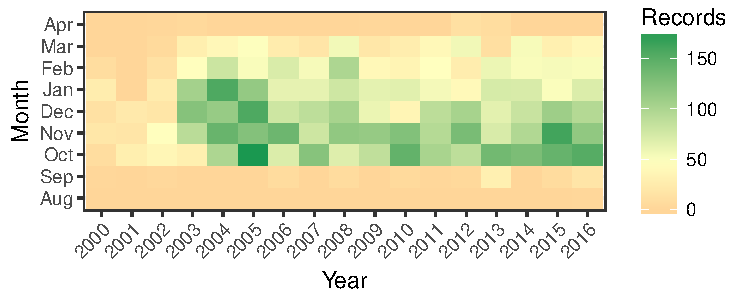
\includegraphics[width = 1.5\linewidth]{data_density.pdf}
\caption{{\small Heatmap of number of flock counts per month in each calendar year. Data are sparse from the early 2000s. Data density is higher in the first three winter months (Oct, Nov, Dec) than the following ones (Jan, Feb, Mar). A mean of 47 flocks are censused per month (range: 0 - 177).}}

\end{figure}

\begin{figure}[H]
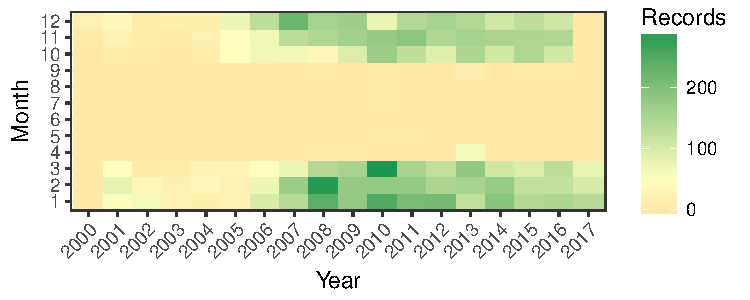
\includegraphics[width = 1.5\linewidth]{data_density_gorg.pdf}
\caption{{\small Heatmap of number of observations of geese marked with numbered neckbands per month in each calendar year. Data are sparse until the mid 2000s. Marked geese are sighted in the study area earlier and later than censused flocks. On average, 49 marked geese are seen each month (range: 0 - 294).}}

\end{figure}

\clearpage

\section{Appendix 2}\label{appendix-2}

\textbf{Model summaries}

We provide tables (Tabs. A1, A2) summarising model structures used in
the analysis. This table includes Cohen's \emph{f\textsuperscript{2}}
effect sizes that are based on the variance explained. Cohen's
\emph{f\textsuperscript{2}} was calculated for each model thus:

\begin{equation} f^2 =  \frac{R^2}{1 - R^2} \end{equation}

where \(R^2\) is the coefficient of determination (Cohen 1988). We
calculated pseudo-\(R^2\) for our models as the \(R^2\) of a linear
model taking the model response of a null generalised mixed model as the
response, and the generalised mixed model fit as the predictor. These
values corresponded closely with pseudo-\(R^2\) provided by the
\emph{mgcv} package for generalised additive models and were considered
reliable as indicators of the variance explained by the model. Cohen's
\emph{f\textsuperscript{2}} values of 0.02, 0.15, and 0.35 are
respectively considered small, medium, and large. Models with a Cohen's
\emph{f\textsuperscript{2}} greater than 1 have an \(R^2\) greater than
0.5.

All models assumed idependent and identically distributed normal
(\emph{iid}) random effects. GLMMs implemented these through their
inbuilt function. GAMMs (models \emph{2.b} and \emph{4}) implemented
random effects as parametric categorical terms penalized by a ridge
penalty (see Wood 2008, 2013).

\begin{table}[H]
\begin{tabular}{l*7l}
\toprule
Model & Type & Dataset & Response & Fixed effects & Random effects & Records used & Cohen's \emph{f\textsuperscript{2}}\\
\midrule
1 & GLMM & B & 6 & 1, 5 & 8, 9, 10 & 20,160\textsuperscript{a}; 14,018\textsuperscript{b} & 3.22\textsuperscript{a}; 4.74\textsuperscript{b}\\

1 & GLMM & C & 6 & 1, 5 & 8, 11 & 3,289\textsuperscript{a}; 7,320\textsuperscript{b} & 4.87\textsuperscript{a}; 4.43\textsuperscript{b}\\

2.a & GLMM & B & 1 & 3, 5, 7 & 8, 9, 10 & 34,179 & 0.09\\

2.a & GLMM & C & 1 & 5, 7 & 8, 11 & 10,426 & 7.72\textsuperscript{c}; 0.62\textsuperscript{d} \\

2.b & GAMM & A & 2 & 3, 5, 7 & 8, 9, 10 & 837 & 9.36\\

3 & GLMM & A & 3 & 5, 6, 7 & 8, 9, 10 & 5,700 & 0.199\\

4 & GAMM & A & 4 & 5, 6, 7 & 8, 9, 10 & 5,659 & 0.52\\\midrule

\multicolumn{8}{l}{\textbf{\emph{Effects}}: \emph{1: Number of juveniles per family, 2: Number of families, 3: Flock size,}} \\
\multicolumn{8}{l}{\emph{4: Proportion of juveniles, 5: Days since autumn arrival,}} \\
\multicolumn{8}{l}{\emph{6: Distance to breeding grounds, 7: Predation index, 8: Breeding year,}} \\
\multicolumn{8}{l}{\emph{9 Observer, 10: Habitat type, 11: Goose identity}} \\
\midrule
\multicolumn{8}{l}{\emph{a: \ensuremath{\le} 60 days after arrival, b: \ensuremath{\ge} 60 days after arrival, c: All families, d: Only successful families}} \\
\bottomrule
\end{tabular}
\caption{Models and inputs based on observation data.}
\end{table}

\begin{table}[H]
\begin{tabular}{l*6l}
\toprule
Model & Type & Response & Fixed effects & Random effects & Records used & Cohen's \emph{f\textsuperscript{2}}\\
\midrule
5.a & GLMM & 1 & 2, 3, 4, 5, 6, 7 & 9 & 1,009\textsuperscript{a} & 0.08 \\

5.b & GLMM & 1 & 3, 8 & 9 & 21,271\textsuperscript{b} & 0.0004\\
\midrule
\multicolumn{6}{l}{\textbf{\emph{Effects}}: \emph{1: Split occurrence , 2: Family size, 3: Days since autumn arrival,}}\\
\multicolumn{6}{l}{\emph{4: Daily number of flights, 5: Cumulative number of previous flights,}}\\
\multicolumn{6}{l}{\emph{6: Daily distance travelled, 7: Cumulative distance previously travelled,}}\\
\multicolumn{6}{l}{\emph{8: Time since last take-off, 9: Family identity}}\\
\midrule
\multicolumn{6}{l}{\emph{a: Daily positions, b: Half-hourly positions}}\\
\bottomrule
\end{tabular}

\caption{Models and inputs based on GPS tracking data.}

\end{table}

\clearpage

\section{Appendix 3}\label{appendix-3}

\textbf{Additional figures}

Here we provide figures referred to in the text.

\begin{figure}[H]
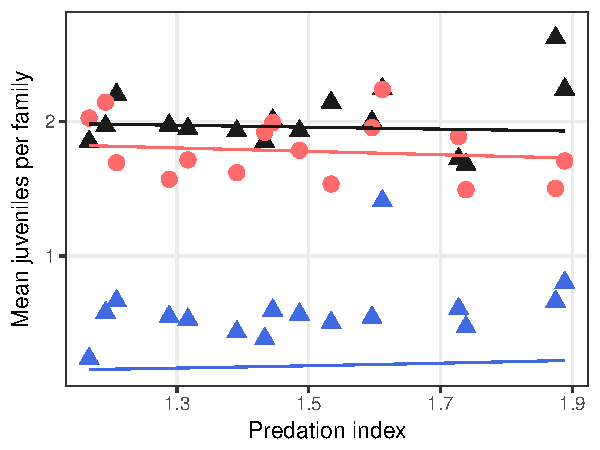
\includegraphics[width = 1\linewidth]{fam_predation.pdf}
\caption{{\small GLMM fits (lines) and mean number of juveniles per family at each
unique level of pooled summer predation index (symbols) using two
datasets: blue, all families of marked geese (dataset \emph{C}); red,
successful families cointed in flocks (dataset \emph{B}); black,
successful families only of marked geese (subset of \emph{C}).}}
\end{figure}

\begin{figure}[H]
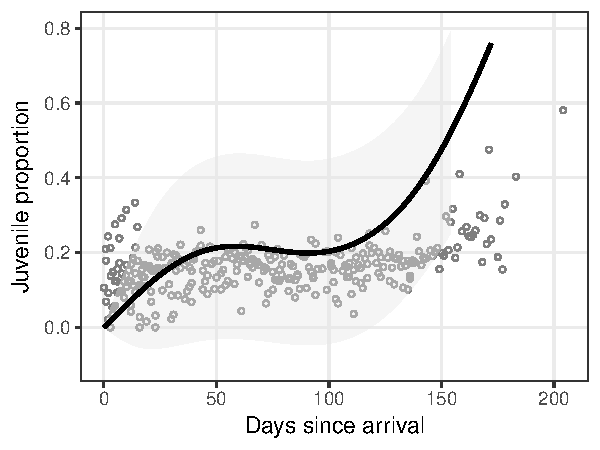
\includegraphics[width = 1\linewidth]{juvprop_time.pdf}
\caption{{\small GAMM partial fit (line) and mean proportion of first-winter juveniles in
white-fronted goose flocks on each winter day, pooled across all years
(circles). Note that days since arrival was modelled as a smoothed
covariate using thin plate splines, and 4 knots. 95\% confidence interval is shaded grey.}}
\end{figure}

\begin{figure}[H]
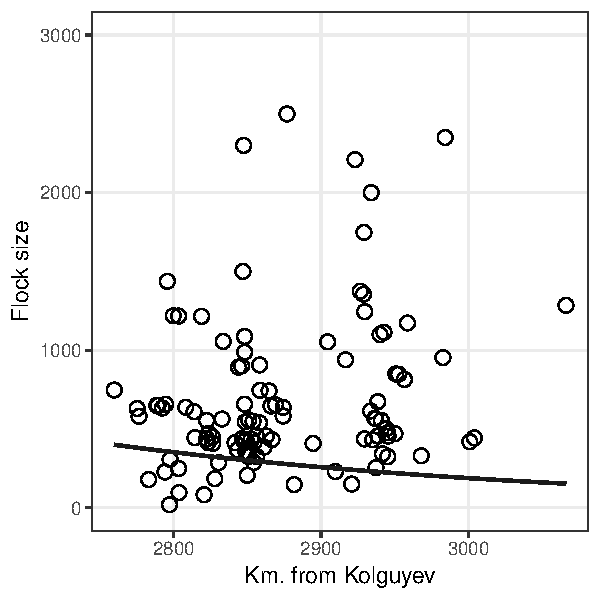
\includegraphics[width = 1\linewidth]{flock_dist.pdf}
\caption{{\small GLMM fit (line) and mean size of flocks at each site (circles, n
= 111) as a function of its distance from Kolguyev Island. Sites to the north-east of the study site are approximately 500 km nearer to Kolguyev than sites in the south-west.}}
\end{figure}

\begin{figure}[H]
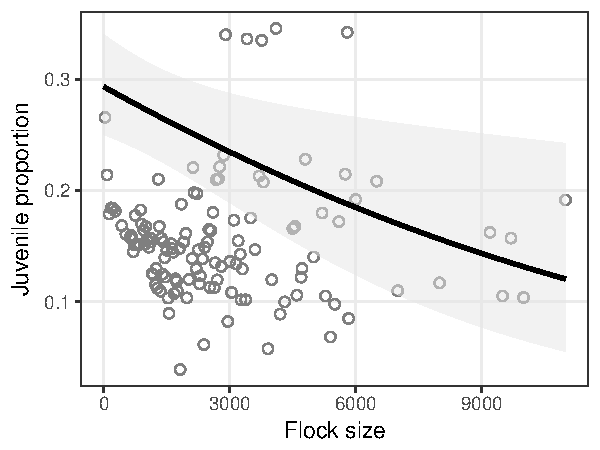
\includegraphics[width = 1\linewidth]{jprop_flock.pdf}
\caption{{\small GAMM fit (line) and mean juvenile proportion of flocks, in increments of 25 individuals (circles). Larger flocks have a lower proportion of juveniles, and lower variance in the proportion. 95\% confidence interval is shaded grey.}}
\end{figure}

\end{document}
